%% -*- fill-column: 79; eval: (auto-fill-mode) -*-
%% vim: tw=79




%\usepackage{authblk}
%% \usepackage{soul}
%% \definecolor{lightyellow}{rgb}{1,1,.60}

%% \mdfsetup{hidealllines=true,backgroundcolor=lightyellow}
%% \sethlcolor{lightyellow}




\lstdefinelanguage{aspx}
{
morekeywords={<\%=,\%>,<\%,<\%:,Username}
}


%% listing settings
\lstset{ %
language=[Sharp]C,                % the language of the code
basicstyle=\footnotesize\ttfamily,       % the size of the fonts that are used for the code
escapeinside={\%*}{*)},         % if you want to add a comment within your code
morekeywords={*,...},           % if you want to add more keywords to
}




\hyphenation{Text-Writer}
\hyphenation{Java-Script}

%% \makeatletter
%% \def\@copyrightspace{\relax}
%% \makeatother

%% \newfont{\mycrnotice}{ptmr8t at 7pt}
%% \newfont{\myconfname}{ptmri8t at 7pt}
%% \let\crnotice\mycrnotice%
%% \let\confname\myconfname%

%% \permission{Permission to make digital or hard copies of all or part of this work for personal or classroom use is granted without fee provided that copies are not made or distributed for profit or commercial advantage and that copies bear this notice and the full citation on the first page. Copyrights for components of this work owned by others than ACM must be honored. Abstracting with credit is permitted. To copy otherwise, or republish, to post on servers or to redistribute to lists, requires prior specific permission and/or a fee. Request permissions from permissions@acm.org.}
%% \conferenceinfo{CCS'13,}{November 4--8, 2013, Berlin, Germany.}
%% \copyrightetc{Copyright 2013 ACM \the\acmcopyr}
%% \crdata{978-1-4503-2477-9/13/11\ ...\$15.00.\\
%% http://dx.doi.org/10.1145/2508859.2516708}

%% \begin{document}

%% \date{}

%% \author{
%% \alignauthor
%% Adam Doup\'e, Weidong Cui, Marcus Peinado, Mariusz H. Jakubowski, Christopher Kruegel, and Giovanni Vigna\\
%% \affaddr{University of California, Santa Barbara  Microsoft Research}
%% \email{testing}
%% }

%% \numberofauthors{6}
%% \author{
%% \alignauthor
%% Adam Doup\'e\\
%% \affaddr{UC Santa Barbara}
%% \email{adoupe@cs.ucsb.edu}
%% \alignauthor
%% Weidong Cui\\
%% \affaddr{Microsoft Research}
%% \email{wdcui@microsoft.com}
%% \alignauthor
%% Mariusz H. Jakubowski\\
%% \affaddr{Microsoft Research}\\
%% \email{mariuszj@microsoft.com}
%% \and
%% \alignauthor
%% Marcus Peinado\\
%% \affaddr{Microsoft Research}\\
%% \email{marcuspe@microsoft.com}
%% \alignauthor
%% Christopher Kruegel\\
%% \affaddr{UC Santa Barbara}\\
%% \email{chris@cs.ucsb.edu}
%% \alignauthor
%% Giovanni Vigna\\
%% \affaddr{UC Santa Barbara}\\
%% \email{vigna@cs.ucsb.edu}
%% }

%% \author[$\S$]{Adam Doup\'e}
%% \author[${\ddag}$]{Weidong Cui}
%% \author[${\ddag}$]{Marcus Peinado}
%% \author[${\ddag}$]{Mariusz H. Jakubowski}
%% \author[$\S$]{Christopher Kruegel}
%% \author[$\S$]{Giovanni Vigna}
%% \affil[$\S$]{University of California, Santa Barbara\\

%% \texttt{\{adoupe, chris, vigna\}@cs.ucsb.edu}}
%% \affil[${\ddag}$]{Microsoft Research\\

%% \texttt{\{wdcui, marcuspe, mariuszj\}@microsoft.com}}

%% \title{deDacota: Toward Preventing Server-Side XSS\\
%%  via Automatic Code and Data Separation}


%% \maketitle

%% %
%  Abstract
%

\begin{abstract}

\addcontentsline{toc}{chapter}{Abstract}

%todo: max 350 words



\abstractsignature

\end{abstract}




%\begin{germanabstract}

%\addcontentsline{toc}{chapter}{Zusammenfassung}

%\end{germanabstract}




%% \category{D.2.5}{Testing and Debugging}{}

%% \keywords{Static Analysis; Cross-Site Scripting; XSS; Content Security Policy; CSP}

%% \pagebreak

\section{Introduction}

Web applications are prevalent and critical in today's computing
world, making them a popular attack target. Looking at types of
vulnerabilities reported in the Common Vulnerabilities and Exposures
(CVE) database~\cite{cve13:overview}, web application flaws are by far
the leading class. 

Modern web applications have evolved into complex programs. These
programs are no longer limited to server-side code that runs on the
web server. Instead, web applications include a significant amount of
JavaScript code that is sent to and executed on the client. Such
client-side components not only provide a rich and fast user
interface, they also contain parts of the application logic and
typically communicate with the server-side component through
asynchronous JavaScript calls. As a result, client-side scripts are
an integral component of modern web applications, and they are
routinely generated by server-side code. 

There are two kinds of cross-site scripting (XSS) vulnerabilities: server-side and
client-side.  The latter is essentially caused by bugs in the
client-side code, while the former is caused by bugs in the
server-side code. In this chapter we focus on server-side XSS vulnerabilities (unless specified
otherwise, we will use XSS to refer to server-side XSS).  XSS vulnerabilities allow attackers to inject
client-side scripting code (typically, JavaScript) into the output of
web applications. The scripts are then executed by the browser as it
renders the page, allowing malicious code to run in the context of the
web application. Attackers can leverage XSS attacks to leak sensitive
user information, impersonate the victim to perform unwanted actions
in the context of the web application, or launch browser exploits.

There has been a significant amount of research effort on
eliminating XSS vulnerabilities. The main line of research has
focused on sanitizing untrusted
input~\cite{yu:10,hooimeijer11:bek,tripp09:taj,livshits05:java-static,weinberger11:sanitization,xie06:static,wassermann07:sound,jovanovic06:pixy-improved,nguyen05:hardening,samuel11:templating,balzarotti08:saner,saxena11:scriptgard,livshits13:automatic-sanitizers,google13:autoescape}.
%
Sanitization attempts to identify and ``clean up'' untrusted inputs
that might contain JavaScript code. Performing correct sanitization is challenging, for a
number of reasons. One reason is that it is difficult to guarantee coverage
for all possible paths through the
application~\cite{balzarotti08:saner,weinberger11:sanitization}. As part
of this problem, it is necessary to find all program locations
(sources) where untrusted input can enter the application, and then
verify, along all program paths, the correctness of all sanitization
functions that are used before the input is sent to the client (sinks). Furthermore,
it is not always clear how to properly sanitize data, because a single input
might appear in different contexts in the output of the application~\cite{saxena11:scriptgard}.

%However, we believe that the need for sanitization is a symptom of and
%not the root cause of XSS vulnerabilities.

The root cause of XSS vulnerabilities is that {\em the current web
  application model violates the principle of code and data
  separation}. In the case of a web page, the data is the HTML content
of the page and the code is the JavaScript code. Mixing JavaScript
code and HTML data in the same channel (the HTTP response) makes it
possible for an attacker to convince a user's browser to interpret
maliciously crafted HTML data as JavaScript code. While sanitization tries to turn untrusted input, which could
potentially contain code, into HTML data,
%Thus, in addition to the
%problems and difficulties with sanitization, attempting to solve the
%sanitization problem is ignoring the root cause of XSS
%vulnerabilities.
%
we believe the fundamental solution to XSS is to %\emph{automatically}
separate the code and data in a web page---the way HTML and JavaScript
should have been designed from the start.  Once the code and data are separated,
a web application can communicate this separation to the browser, and the
browser can ensure no code is executed from the data channel.
Such communication and enforcement is supported by the new W3C browser standard
Content Security Policy (CSP)~\cite{stamm10:csp}.

While new web applications can be designed with code and data
separated from the start, it has been a daunting task to achieve code
and data separation for legacy applications. The key challenge is to
identify code or data in the output of a web application. Previous
solutions have relied on either developers' manual annotations or
dynamic analysis. For example, BEEP~\cite{jim07:beep} requires
developers to manually identify inline JavaScript code. {\sc
  Blue\-print}~\cite{louw09:blueprint} requires developers to manually
identify the data by specifying which application statements could
output untrusted input. XSS-GUARD dynamically identifies
application-intended JavaScript code in a web page by comparing it
with a shadow web page generated at run time~\cite{bisht08:xssguard}. The main problem
preventing these solutions from being adopted is either the
significant manual effort required from application developers or the
significant runtime performance overhead. In fact, Weinberger et
al.~\cite{weinberger11:client} showed how difficult it is to manually
separate the code and data of a web application.

%There has been some research in this direction; research that attempts
%to restrict the client-side code execution of the web
%application to only known scripts. BEEP~\cite{jim07:beep} enables the
%developer to specify a \emph{manually} developed policy about which
%scripts to execute, and then a modified browser will execute only
%those policies. {\sc Blueprint}~\cite{louw09:blueprint} will execute
%only intended JavaScript code, without browser modification and
%resistant to browser parsing quirks. However, a developer must
%\emph{manually} identify statements in the server-side code that
%output untrusted data, which is essentially sanitization
%(if a developer can identify all statements that output untrusted
%data, then they can sanitize properly).
%
%The main problem preventing these solutions from being adopted is the
%manual effort required by the developer. BEEP requires the developer
%to identify all inline scripts manually (with a hash) and {\sc
%  Blueprint} requires the developer to find all statements that output
%untrusted data. In fact, Weinberger et al.~\cite{weinberger11:client}
%showed how difficult it is to manually separate the code and data of a
%web application.

In this chapter, we present \dedacota, the first system that can
automatically and statically rewrite an existing web application to separate code and
data in its web pages. Our novel idea is to use static analysis to
determine all inline JavaScript code in the web pages of an application. 
Specifically, \dedacota performs static data-flow analysis of a given
web application to approximate its HTML output. Then, it parses each page's
HTML output to identify inline JavaScript code. Finally, it rewrites
the web application to output the identified JavaScript code in a
separate JavaScript file.

%As being able to statically determine, both soundly and completely, all
%possible HTML output of a web application is undecidable (it is
%equivalent to the halting problem), \dedacota attempts to automate as
%much as possible while at the same time alerting the developer when it
%makes a mistake.

%Theoretically, the HTML output of a web application is undecidable
%because it is equivalent to the halting problem. However, in practice
%we deal with benign applications which makes the problem more
%tractable. For instance, the majority of the inline JavaScript code is
%constant. Furthermore, code and data separation will eliminate XSS
%vulnerabilities when the code section is static. Modern web
%application, however, frequently contain JavaScript that is
%dynamically generated by server-side code. A XSS vulnerability can
%still be present if an attacker can inject unsanitized JavaScript into
%the code section of the application. Thus, while \dedacota aims to
%fully automatically separate the code and data of a web application,
%there are classes of XSS vulnerabilities that will remain in the
%application after the transformation.

The problem of statically determining the set of (HTML) outputs of a web
application is undecidable. However, as we observe in our evaluation, the
problem is typically tractable for real-world web applications. These
applications are written by benign developers and tend to have special
properties that allow us to compute their outputs statically. For instance, the
majority of the inline JavaScript code is static in the web applications we
tested.

Dynamic inline JavaScript presents a second-order problem. Here, the JavaScript
code itself (rather than the HTML page) is generated dynamically on the server
and may depend on untrusted inputs. Again, the potential
for XSS vulnerabilities exists. \dedacota provides a partial solution to this
problem by producing alerts for all potentially dangerous instances of dynamic
JavaScript generation in the application and by safely sanitizing a large
subclass of these instances.

%% Furthermore, we also opt to trigger
%% an alert when our static analysis cannot decide the rewriting operations.
%% For the web applications we tested, the alerts are controlled under 5.

%Now that the code and data of the web
%application have been separated, we can leverage the new W3C browser
%standard Content Security Policy (CSP)~\cite{stamm10:csp} to enforce
%this separation and ensure that no code is executed in the data
%channel. 

%We believe that this approach to preventing XSS vulnerabilities, in
%addition to solving the root of the problem, has advantages over
%sanitization. Static sanitization approaches must find \emph{all}
%places that can output untrusted code throughout the application,
%whereas our approach attempts to find all inline JavaScript code. Even
%though both approaches use static analysis, and are prone to the same
%problems, we argue that our approach is, in some sense, more tractable
%than the sanitization problem, because our approach needs to discover
%``less'' of the application.

%% Moreover, any practical solution must be automated, to be
%% applicable to the huge number of legacy web applications. Once code
%% and data in a web page are separated, we can use browser enhancements,
%% such as CSP, to enforce this distinction and prevent attackers from
%% injecting JavaScript code as HTML data.

%% There has been a significant amount of research efforts on ways to
%% eliminate XSS vulnerabilities. They generally fall into two
%% categories: Sanitizing untrusted input or specifying trusted
%% JavaScript code. The goal of the first line of research is to identify
%% and ``clean up'' untrusted inputs that might contain JavaScript code
%% and then end up in the output of the application. Performing correct
%% sanitization is challenging, for a number of reasons. One is that it
%% is difficult to guarantee coverage for all possible application
%% paths~\cite{balzarotti08:saner,weinberger11:sanitization}. As part of
%% this problem, it is necessary to find all program locations (sources)
%% where untrusted inputs can enter the application, and one has to
%% verify the correctness of all sanitization functions that are used.
%% Another problem is that it is not always clear how to properly
%% sanitize data, because it might appear in different contexts in the
%% output of the application~\cite{saxena11:scriptgard}. As a result,
%% automated sanitization approaches often focus on particular templating
%% languages that make the analysis process
%% feasible~\cite{samuel11:templating,google13:autoescape}.

%% Recent automatic XSS sanitization solutions are limited to either
%% incomplete execution path coverage~\cite{} or applications written in
%% a specific templating language~\cite{}.This approach have limited
%% applicability because performing correct sanitization is challenging
%% due to ambiguous contexts for parsing untrusted input~\cite{}.

We implemented a prototype of \dedacota to analyze and rewrite
ASP.NET~\cite{asp-dot-net} web applications. We applied \dedacota
to six open-source, real-world ASP.NET applications.
%By design, our system eliminates almost all server-side XSS vulnerabilities.
We verified that all known XSS vulnerabilities are eliminated. We then
performed extensive testing to ensure that the rewritten binaries
still function correctly.  We also tested \dedacota's performance and found that the
page loading times between the original and rewritten application are
indistinguishable.

%Our novel idea is that we can prevent XSS vulnerabilities by separating the
%JavaScript code from the HTML data and that this separation can be done
%automatically. Then, using a mechanism on the browser to enforce this
%separation, an attacker cannot trick the browser into interpreting HTML data as
%JavaScript code. Thus, using this approach, we can automatically protect web
%applications from a wide swath of XSS vulnerabilities (in
%Section~\ref{xss-background} we discuss exactly what types of XSS
%vulnerabilities our approach prevents).

%\textbf{Possibly move this paragraph to later section.} With regards to code and
%data separation of the web page, the problem can be simplified to that of not
%using inline JavaScript. Once again, this is because the browser cannot tell if
%the application developer intended for the inline JavaScript to be executed or
%if the inline JavaScript came from a malicious user. Thus, our goal is to
%statically locate every inline JavaScript in the web application and rewrite it
%to be an external JavaScript. We then rely on a new browser feature called
%Content Security Policy (CSP) to prevent any inline JavaScript from executing.

\smallskip \noindent{}The main contributions of this chapter are the following:

\begin{itemize}
% Is this really new?
%\item  A novel way of looking at cross-site scripting vulnerabilities as
 % intermixing of code and data in the same channel (Section~\ref{background}).
\item A novel approach for automatically separating the code and data
  of a web application using static analysis (Section~\ref{design}).
\item A prototype implementation of our approach, \dedacota, applied to ASP.NET applications
(Section~\ref{implementation}).
\item An evaluation of \dedacota, showing that we are able to apply
  our analysis to six real-world, open-source, ASP\-.NET applications. We show that
  our implementation prevents the exploitation of know vulnerabilities and that
  the semantics of the application do not change (Section~\ref{evaluation}).
\end{itemize}

\section{Background}
\label{background}

In this section, we provide the background necessary for understanding
the design of \dedacota.

%Before delving into how our Cross-Site Scripting (XSS) prevention system works,
%we must first make two issues clear: (1) What type of XSS vulnerabilities our
%system targets, and (2) how separation of code and data can be applied to the
%web context.

\subsection{Cross-Site Scripting}
\label{xss-background}

Modern web applications consist of both server-side and client-side
code.  Upon receiving an HTTP request, the server-side code, which is
typically written in a server-side language, such as PHP or ASP.NET, dynamically
generates a web page as a response, based on the user input in the
request or data in a backend database.  The client-side code,
which is usually written in JavaScript and is executed by the browser, can be either inline in the
web page or external as a standalone JavaScript file.

Cross-site scripting (XSS) vulnerabilities allow an attacker to inject
malicious JavaScript into web pages to execute in the client-side
browser, as if they were generated by the trusted web site. If the vulnerability
allows the attacker to store malicious JavaScript on the server (e.g.,
using the contents of a message posted on a newsgroup), the
vulnerability is traditionally referred to as ``stored'' or
``persistent XSS.'' When the malicious code is included in the request
and involuntarily reflected to the user (copied into the response) by
the server, the vulnerability is called ``reflected XSS.'' Finally, if
the bug is in the client-side code, the XSS vulnerability is referred
to as ``DOM-based XSS''~\cite{klein05:dom-xss}. We call the first two types of
vulnerabilities ``server-side XSS vulnerabilities'' and the latter
``client-side XSS vulnerabilities.'' 
%% In the rest of this chapter, we use
%% ``XSS'' and ``XSS vulnerabilities'' interchangeably.

The root cause for server-side XSS is that the code (i.e., the
client-side script) and the data (i.e., the HTML content) are mixed
together in a web page.  By crafting some malicious input that will be
included into the returned web page by the server-side code, an
attacker can trick the browser into confusing his data as JavaScript
code.

%Cross-Site Scripting vulnerabilities continue to plague web
%applications
%\textbf{Cite}. In fact, they are the most frequent vulnerabilities currently
%being exploited on the Internet today.

%The browser security mechanism Same Origin Policy (SOP) prevents JavaScript
%from different websites from interacting and interfering with each other. For
%instance, the malicious JavaScript from \texttt{evil.com} cannot, when loaded
%and executed from \texttt{evil.com}, affect the integrity of
%\texttt{goodsite.com}. 

%A XSS vulnerability occurs when a malicious is able to trick a web application
%into including JavaScript of the attacker's choosing in the web page response.
%Thus, a user browsing the web page would execute the attacker's JavaScript. By
%executing the JavaScript of his choosing, a malicious user can do a number of
%actions, four of which are discussed here. (1) An attacker can steal the
%cookies of the user to the web application, using those cookies to log into the
%application as the user. (2) The attacker can manipulate the application on
%behalf of the user, bypassing any Cross-Site Request Forgery\textbf{cite}
%defenses. (3) The attacker can attempt to exploit the user's browser and thus
%infect the user's computer. (4) The attacker can completely control the layout
%and look of the web page, so they can create a fake login screen to phish the
%user's username/password.

%\para{Classic types of XSS vulnerabilities. 1st order, 2nd order, 3rd order}

%\para{New classification based on \emph{where} the vulnerability occurs}

%\subsubsection{Server-Side}

%\para{The vulnerability is the result of a bug in the server-side code}

%\para{Can be either 1st order or 2nd order.}

%\subsubsection{Client-Side}

%\para{The vulnerability is the result of a bug in the JavaScript code}

%\para{Obviously, only 3rd order}

%\para{Our approach will only fix server-side XSS vulnerabilities. Other
%  techniques must be used to fix client-side XSS vulnerabilities.}

\subsection{Code and Data Separation}

The separation of code and data can be traced back to the Harvard
Architecture, which introduces separate storage and buses for code and
data. Separating code and data is a basic security principle for
avoiding code injection attacks~\cite{howard03:secure-code}. Historically,
whenever designs violate this principle, there exists a security hole.
An example is the stack used in modern CPUs. The return addresses
(code pointers) and function local variables (data) are co-located on
the stack. Because the return addresses determine control transfers,
they are essentially part of the code. Mixing them together with the
data allows attackers to launch stack overflow attacks, where data
written into a local variable spills into an adjacent return address.
In the context of web applications, we face the same security
challenge, this time caused by mixing code and data together in web
pages. To fundamentally solve this problem, we must separate code and
data in web pages created by web applications.

%\para{The general idea of code and data separation along with references to the
%  original papers.}

%\subsubsection{Previous Code and Data Separation}

%\para{Talk about previous applications of Code and Data Separation. Binary.}

%\subsubsection{Code and Data Separation applied to Web Applications}

%\para{Reiterate the claim that XSS vulnerabilities (and indeed, SQL injection
%  vulnerabilities) root cause the mixing of code and data}

\subsection{Content Security Policy}

Content Security Policy (CSP)~\cite{stamm10:csp} is a mechanism for
mitigating a broad class of content injection vulnerabilities in web
applications.  CSP is a declarative policy that allows a web
application to inform the browser, via an HTTP header,
about the sources from which the application expects to load resources
such as JavaScript code.  A web browser that implements support
for CSP can enforce the security policy declared by the web
application.

A newly developed web application can leverage CSP to avoid XSS by not
using inline JavaScript and by specifying that only scripts from a set of
trusted sites are allowed to execute on the client. Indeed, Google has
required that all Chrome browser extensions implement
CSP~\cite{akhawe12:privilege}. However, manually applying CSP to a
legacy web application typically requires a non-trivial amount of
work~\cite{weinberger11:client}. The reason is that the authors of the
web application have to modify the server-side code to clearly
identify which resources (e.g., which JavaScript programs) are used by
a web page. Moreover, these scripts have to be separated from the web
page.

CSP essentially provides a mechanism for web browsers to enforce the
separation between code and data as specified by web applications.
Our work solves the problem of automatically transforming legacy web
applications so that the code and data in their web pages are
separated. The transformed web applications can then directly leverage
the browser's support for CSP to avoid a wide range of XSS
vulnerabilities.

%\para{CSP is the mechanism to enforce code and data separation.}

%\para{CSP is hard to implement manually (cite workshop paper).}

%Possibly need a figure with CSP header and explanation of the header. 

\section{Threat Model}
\label{threat-model}

Before discussing the design of \dedacota, we need to state our assumptions
about the code that we are analyzing and the vulnerabilities we are addressing.

Our approach involves rewriting a web application. This web application is
written by a benign developer---that is, the developer has not intentionally
obfuscated the code as a malicious developer might. This assumption
also means that the JavaScript and HTML are benign and not intentionally taking
advantage of browser parsing quirks (as described in {\sc Blue\-print}~\cite{louw09:blueprint}).

%%  attackers input malformed
%% HTML that some browsers, due to the leniency of their parsers, will interpret
%% and execute as JavaScript. An example of this malformed input is:\\
%% \texttt{<b
%%   <script>alert(1)//</script>0</script></b>} which will execute in some
%% versions of Firefox, Chrome, and
%% Safari\footnote{\url{http://heideri.ch/jso/\#59}}.

\dedacota will only prevent \emph{server-side} XSS vulnerabilities. We define
server-side XSS vulnerabilities as XSS vulnerabilities where the \emph{root
  cause} of the vulnerability is in server-side code. Specifically, this means
XSS vulnerabilities where unsanitized input is used in an HTML page. We
explicitly do not protect against client-side XSS vulnerabilities, also called
DOM-based XSS. Client-side XSS vulnerabilities occur when untrusted input is
interpreted as JavaScript by the client-side JavaScript code using methods such
as \texttt{eval}, \texttt{document.write}, or \texttt{innerHTML}. The root
cause of these vulnerabilities is in the \emph{JavaScript code}.

In this chapter, we focus solely on separating inline JavaScript code (that is, JavaScript
in between {\tt <script>} and {\tt </script>}). While there are other vectors
where JavaScript can be executed, such as JavaScript code in HTML attributes
(event handlers such as {\tt onclick}) and inline Cascading Style Sheet (CSS)
styles~\cite{heiderich12}, the techniques described here can be
extended to approximate and rewrite the HTML attributes and inline CSS.

Unfortunately, code and data separation in an HTML page is not a panacea for
XSS vulnerabilities. In modern web applications, the inline JavaScript code is
sometimes dynamically generated by the server-side code. A common scenario is
to use the dynamic JavaScript code to pass data from the server-side code to
the client-side code.
There may be XSS vulnerabilities, even if code and data are properly separated,
if the data embedded in the JavaScript code is not properly sanitized.
\dedacota provides a partial solution to the problem of dynamic JavaScript (see
Section~\ref{dynamic-inline-javascript}).
% If the code section is completely static, then a properly
%separated application will be immune to XSS vulnerabilities. In modern web
%applications, however, this is frequently not the case. The server-side code
%can be used to dynamically generate JavaScript (the common situation is to
%pass data from the server-side code to the client-side code at request time).
%Although \dedacota cannot handle all cases of dynamic JavaScript, we have made
%a first step in this direction by handling the common case when 
%passing data from
%the server-side code to the JavaScript in a string.
%The details of this approach are in Section~\ref{dynamic-inline-javascript}.
\section{Design}
\label{design}

Our goal is to statically transform a given web application so that the new
version preserves the application semantics but outputs web pages where all the
inline JavaScript code is moved to external JavaScript files. These external
files will be the \emph{only} JavaScript that the browser will execute, based
on a Content Security Policy. 

There are three high-level steps to our approach.  For each web page
in the web application: (1) we statically determine a conservative
approximation of the page's HTML output, (2) we extract all
inline JavaScript from the approximated HTML output, and (3) we rewrite
the application so that all inline JavaScript is moved to external
files.  

Hereinafter, we define a running example that we use to describe how
\dedacota automatically transforms a web application, according to the
three steps outlined previously.

%approach attempts to automatically separate the JavaScript
%code from the HTML data of a web application, with the goal of increasing the
%security of the application by eliminating server-side Cross-Site
%Scripting (XSS) vulnerabilities.

%Our algorithm takes in a web application (our prototype implementation,
%explained in Section~\ref{implementation}, targets ASP.NET binaries) and
%outputs a transformed version of that application. This transformed version has
%the inline JavaScript rewritten to external JavaScript.

%However, as we shall see, our approach is general, and is not constrained to
%any specific server-side programming language.

%\subsection{Goals}

%There are multiple design goals that our approach must follow: we want to
%increase the security of the web application, however we want to preserve the
%semantics of the web application as well. This means that we must be
%conservative in our approach of what to rewrite and how to rewrite the web
%application.

%In order to show that our approach has merit, in this paper we focus on
%removing and rewriting inline JavaScript (JavaScript in between
%\texttt{<script>} and \texttt{</script>}). To be completely safe from
%server-side XSS vulnerabilities, one must also separate JavaScript code in
%HTML attributes (event handlers, such as \texttt{onclick}), and even inline
%Cascading Style Sheets (CSS) styles~\cite{heiderich12}. Our approach is not confined
%to simply inline JavaScript, and it can be easily extended to JavaScript
%attributes and CSS styles.

%% The question arises, why approach the web application in this way? What is
%% wrong with existing techniques that attempt to find all possible paths in the
%% application where untrusted user input is output to the user without proper
%% sanitization. It turns out that this solution is fraught with complications.
%% Prateek et al.\ \textbf{cite} demonstrated that getting the sanitization of
%% output is difficult, because the specific type of sanitization needed depends
%% on where the output is located in the HTML context of the web page.
%% Furthermore, typical static analysis approaches will either miss possible
%% vulnerabilities due to dynamic code execution (false negatives) or will report
%% many non-existent vulnerabilities (false positives).

%% With our approach, we attempt to solve a simpler problem. We statically
%% identify all inline JavaScript in the application. Our theory is that,  it
%% should be possible to statically determine all inline JavaScript in the
%% application. The intuition here is that developers, who write web applications,
%% do not write complicated or statically undeterminable application code that
%% outputs inline JavaScript. The problem being that there is a high cost to
%% maintain such complicated application code.

%%%%%%%%%%%%%%%%%%%%%%%%%%%%%%%%%%%%%%%%%%%%%%%%%%%%%%%%%%%%%%%%%%%%%%%%%%%%%%%%
\subsection{Example}

Listing~\ref{code:simple-aspx} shows a simplified ASP.NET Web Form page.
Note that everything not in between the \opentag and \closetag is output
directly to the browser. Everything between matching \opentag and
\closetag is \csh code. A subtle but important point
is that \opentageq is used to indicate that the \csh code will output a
string at that location in the HTML output.

\begin{lstlisting}[language=aspx, caption=Example of a simple ASP.NET Web Form page., label=code:simple-aspx, float]
<html>
  <% Title = "Example";
	 Username = Request.Params["name"]; %>
  <head><tile><%= Title %></title></head>
  <body>
    <script>
      var username = "<%= Username %>";
    </script>
  </body>
</html>
\end{lstlisting}




In Listing~\ref{code:simple-aspx}, Line~2 sets the title of the page, and
Line~3 sets the \texttt{Username} variable to the \texttt{name} parameter
sent in the query string. The \texttt{Username} is output to the browser inside
a JavaScript string on Line~7. This is an example of the \csh server-side code
passing information to the JavaScript client-side code, as the intent here is
for the JavaScript \texttt{username} variable to have the same value as the
\csh \texttt{Username} variable.


Internally, ASP.NET compiles the ASP.NET Web Form page to \csh, either when
the application is deployed, or on-demand, as the page is accessed. The
relevant compiled \csh output of Listing~\ref{code:simple-aspx} is shown in
Listing~\ref{code:simple-compiled-cs}. Here, the ASP.NET Web Form page has been
transformed into an equivalent \csh program. The ASP.NET compiler creates a
class (not shown) that represents the ASP.NET Web Form. A
method of the class is given a \texttt{TextWriter} object as a parameter.
Anything written to this object will be sent in the HTTP response.
\texttt{TextWriter.Write} is a method call equivalent of writing to the console
in a traditional command-line application.

\begin{lstlisting}[language={[Sharp]C}, caption=The compiled \csh output of Listing~\ref{code:simple-aspx}., label=code:simple-compiled-cs, float]
void Render(TextWriter w) {
  w.Write("<html>\n  ");
  this.Title = "Example";
  this.Username = Request.Params["name"];
  w.Write("\n  <head><tile>");
  w.Write(this.Title);
  w.Write("</title></head>\n  <body>\n    <script>\n      var username = \"");
  w.Write(this.Username);
  w.Write("\";\n    </script>\n  </body>\n</html>");
}
\end{lstlisting}


From comparing Listing~\ref{code:simple-aspx} to
Listing~\ref{code:simple-compiled-cs}, one can see that output not between
\opentag and \closetag tags is written to the \texttt{TextWriter} object. The
code between the \opentag and \closetag tags is inlined into the function
(Lines~3 and 4), and the code that is between the \opentageq and \closetag tags
is written to the \texttt{TextWriter} object (Lines~6 and 8). We also
note that \dotwrite is one of a set of methods used to write content to
the HTTP response. However, for simplicity, in the remainder of this chapter, we will
use \dotwrite to represent all possible ways of writing content to the HTTP
response.

%Now that we have some idea of how a web application generates its output, let us
%look at a high-level overview of our algorithm.

%%%%%%%%%%%%%%%%%%%%%%%%%%%%%%%%%%%%%%%%%%%%%%%%%%%%%%%%%%%%%%%%%%%%%%%%%%%%%%%%
\subsection{Approximating HTML Output}

In the first phase of our approach, we approximate the HTML output of a web
page. This approximation phase is a two-step process. First, we need to determine, at every
\dotwrite location, what is being written. Second, we need to determine the
order of the \dotwrite{} function invocations.

We use a different static analysis technique to answer each of the two
questions. To determine what is being written at a \dotwrite, we use the
points-to analysis algorithm presented in~\cite{cui12:tracking} modified to work
on .NET byte-code, instead of C. This points-to analysis algorithm is
inclusion-based, demand-driven, context-sensitive, field-sensitive, and
partially flow-sensitive. The points-to analysis algorithm computes the set of
strings that alias with the parameter of \dotwrite. If all strings in the alias
set are constant strings, the output at the \dotwrite will be defined as the
conjunction of all possible constant strings. Otherwise, we say the output is
statically undecidable.
%
%The pointer analysis will either give us the set of constant strings if the
%variable can only be those constant strings or tell us that the variable can be
%anything.
To determine the ordering of all \dotwrite method calls, we build a
control-flow graph, using standard techniques, that only contains the
\dotwrite{} method calls.

\begin{figure}[tb]
  \centering
  \resizebox{0.8\textwidth}{!}{
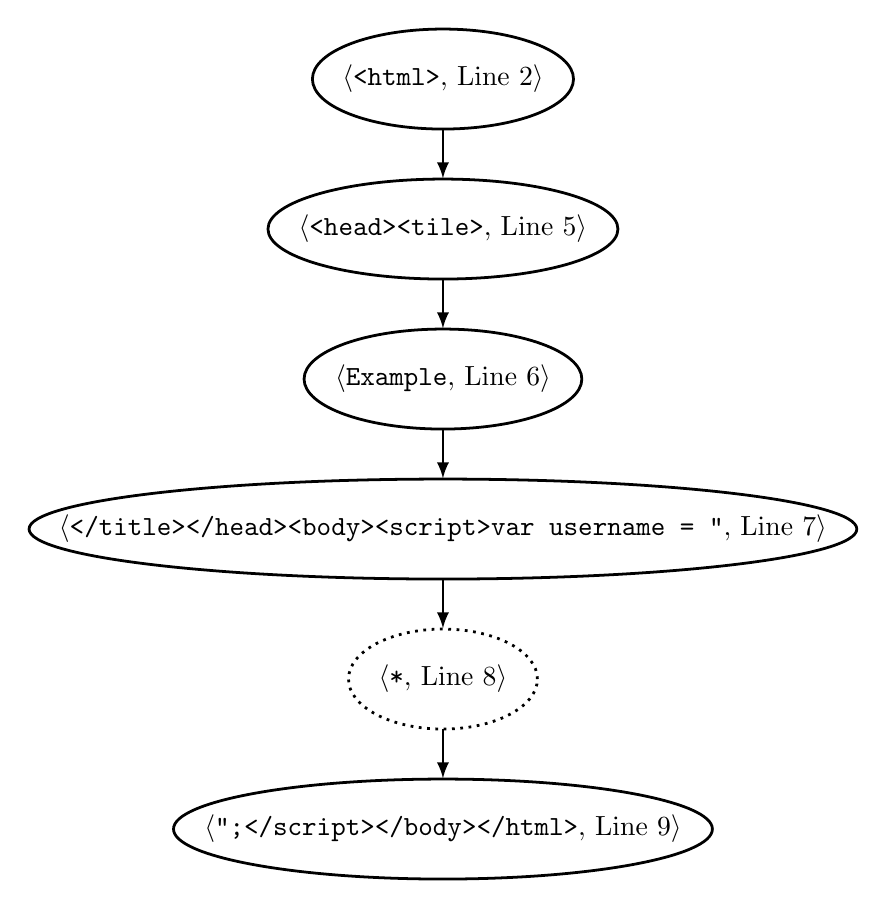
\begin{tikzpicture}[>=latex,line join=bevel,]
  \pgfsetlinewidth{1bp}
%%
\pgfsetcolor{black}
  % Edge: 5 -> 6
  \draw [->] (149bp,53.973bp) .. controls (149bp,51.574bp) and (149bp,49.059bp)  .. (149bp,36.243bp);
  % Edge: 1 -> 2
  \draw [->] (149bp,269.97bp) .. controls (149bp,267.57bp) and (149bp,265.06bp)  .. (149bp,252.24bp);
  % Edge: 4 -> 5
  \draw [->] (149bp,107.97bp) .. controls (149bp,105.57bp) and (149bp,103.06bp)  .. (149bp,90.243bp);
  % Edge: 2 -> 3
  \draw [->] (149bp,215.97bp) .. controls (149bp,213.57bp) and (149bp,211.06bp)  .. (149bp,198.24bp);
  % Edge: 3 -> 4
  \draw [->] (149bp,161.97bp) .. controls (149bp,159.57bp) and (149bp,157.06bp)  .. (149bp,144.24bp);
  % Node: 1
\begin{scope}
  \definecolor{strokecol}{rgb}{0.0,0.0,0.0};
  \pgfsetstrokecolor{strokecol}
  \draw (149bp,288bp) ellipse (47bp and 18bp);
  \draw (149bp,288bp) node {$\langle$\texttt{<html>}$,$ Line 2$\rangle$};
\end{scope}
  % Node: 3
\begin{scope}
  \definecolor{strokecol}{rgb}{0.0,0.0,0.0};
  \pgfsetstrokecolor{strokecol}
  \draw (149bp,180bp) ellipse (50bp and 18bp);
  \draw (149bp,180bp) node {$\langle$\texttt{Example}$,$ Line 6$\rangle$};
\end{scope}
  % Node: 2
\begin{scope}
  \definecolor{strokecol}{rgb}{0.0,0.0,0.0};
  \pgfsetstrokecolor{strokecol}
  \draw (149bp,234bp) ellipse (63bp and 18bp);
  \draw (149bp,234bp) node {$\langle$\texttt{<head><tile>}$,$ Line 5$\rangle$};
\end{scope}
  % Node: 5
\begin{scope}
  \pgfsetdash{{\pgflinewidth}{2pt}}{0pt}
  \definecolor{strokecol}{rgb}{0.0,0.0,0.0};
  \pgfsetstrokecolor{strokecol}
  \draw [dotted] (149bp,72bp) ellipse (34bp and 18bp);
  \draw (149bp,72bp) node {$\langle$\texttt{*}$,$ Line 8$\rangle$};
\end{scope}
  % Node: 4
\begin{scope}
  \definecolor{strokecol}{rgb}{0.0,0.0,0.0};
  \pgfsetstrokecolor{strokecol}
  \draw (149bp,126bp) ellipse (149bp and 18bp);
  \draw (149bp,126bp) node {$\langle$\texttt{</title></head><body><script>var username = \symbol{34}}$,$ Line 7$\rangle$};
\end{scope}
  % Node: 6
\begin{scope}
  \definecolor{strokecol}{rgb}{0.0,0.0,0.0};
  \pgfsetstrokecolor{strokecol}
  \draw (149bp,18bp) ellipse (97bp and 18bp);
  \draw (149bp,18bp) node {$\langle$\texttt{\symbol{34};</script></body></html>}$,$ Line 9$\rangle$};
\end{scope}
%
\end{tikzpicture}

}
  \caption{Approximation graph for the code in
    Listing~\ref{code:simple-aspx} and
    Listing~\ref{code:simple-compiled-cs}. The dotted node's content
    is not statically determinable. }
  \label{simple-approximation-graph}
\end{figure}


We encode the information produced by the two static analyses---the ordering of \dotwrite method calls and their
possible output---into a graph that we call an \emph{approximation graph.}
Figure~\ref{simple-approximation-graph} shows the approximation graph for the
code in Listing~\ref{code:simple-aspx} and
Listing~\ref{code:simple-compiled-cs}. Each node in the graph contains
the location of the \dotwrite that this node represents as well as the possible constant
strings that could be output at this \dotwrite location. Content that cannot be
determined statically is represented by a wild card \texttt{*} (the dotted node in
Figure~\ref{simple-approximation-graph}).
The strings that may be output at the \dotwrite will be used to identify inline
JavaScript, and the location of the \dotwrite will be used for rewriting the
application.

\begin{figure}[tb]
  \centering
  \resizebox{0.80\textwidth}{!}{
\begin{tikzpicture}[>=latex,line join=bevel,]
%%
\node (1) at (206bp,208bp) [draw,ellipse] {$\langle$\texttt{<script>}$,$ Line 20$\rangle$};
  \node (3) at (328bp,170bp) [draw,ellipse] {$\langle$\texttt{setupGuest();}$,$ Line 30$\rangle$};
  \node (2) at (85bp,170bp) [draw,ellipse] {$\langle$\texttt{setupAdmin();}$,$ Line 30$\rangle$};
  \node (5) at (130bp,91bp) [draw,ellipse,line width=3pt, dotted] {$\langle$\texttt{*}$,$ Line 50$\rangle$};
  \node (4) at (206bp,131bp) [draw,ellipse,line width=3pt] {$\langle$\texttt{var test = \symbol{34}}$,$ Line 40$\rangle$};
  \node (7) at (206bp,12bp) [draw,ellipse] {$\langle$\texttt{</script>}$,$ Line 70$\rangle$};
  \node (6) at (206bp,51bp) [draw,ellipse,line width=3pt] {$\langle$\texttt{\symbol{34};}$,$ Line 60$\rangle$};
  \draw [->] (5) ..controls (158.43bp,75.784bp) and (167.28bp,71.359bp)  .. (6);
  \draw [->] (6) ..controls (206bp,36.789bp) and (206bp,35.659bp)  .. (7);
  \draw [->] (4) ..controls (175.52bp,114.76bp) and (167.41bp,110.7bp)  .. (5);
  \draw [->] (1) ..controls (252.39bp,193.31bp) and (269.01bp,188.41bp)  .. (3);
  \draw [->] (6) ..controls (207.48bp,68.519bp) and (207.83bp,73.476bp)  .. (208bp,78bp) .. controls (208.44bp,89.547bp) and (208.44bp,92.453bp)  .. (208bp,104bp) .. controls (207.96bp,105.13bp) and (207.9bp,106.29bp)  .. (4);
  \draw [->] (1) ..controls (160.13bp,193.35bp) and (143.82bp,188.5bp)  .. (2);
  \draw [->] (3) ..controls (281.36bp,154.86bp) and (265.84bp,150.15bp)  .. (4);
  \draw [->] (2) ..controls (131.25bp,154.86bp) and (146.65bp,150.15bp)  .. (4);
%
\end{tikzpicture}

}
  \caption{Approximation graph with branches and a loop. The loop will
  be collapsed into one node to create the final approximation graph.}
  \label{complex-graph}
\end{figure}


%While the approximation graph in Figure~\ref{simple-approximation-graph} is
%simple, too simple to be representative of a majority of programs,
In Figure~\ref{complex-graph} we show the approximation graph of a more complex
page. The graph in Figure~\ref{complex-graph} contains a branch, where each node in the
branch maps to the same \dotwrite method. This happens when the points-to
analysis says that the \dotwrite method can output one of multiple strings. The
other way there can be a branch in the approximation graph is when there is a
branch in the control flow of the web application. The
graph in 
Figure~\ref{complex-graph} also contains a loop that includes the nodes shown
in bold. However,
because we cannot statically determine the number of times a loop may execute,
and we want our analysis to be conservative, we collapse all
nodes of a loop (in the approximation graph) into a single node. This new node now has
%\textbf{adam: possibly create diagram}
undecidable content (represented by a \texttt{*}). The new node also
keeps track of all the \dotwrite methods that were part of the original loop.

After collapsing all loops in the graph, we derive a conservative approximation
of the HTML output of a web page. The approximation graph is a directed
acyclic graph (DAG), and any path from the root node to a leaf node will
represent one possible output of the web page.


%%%%%%%%%%%%%%%%%%%%%%%%%%%%%%%%%%%%%%%%%%%%%%%%%%%%%%%%%%%%%%%%%%%%%%%%%%%%%%%%
\subsection{Extracting Inline JavaScript}
\label{extracting}

In the second phase, our approach uses the approximation graph described
previously to extract all possible inline JavaScript. The
output of this phase is a set containing all possible inline JavaScript that
may appear in the web page.
%, along with, for every
%inline JavaScript, the associated metadata (what parts of the inline JavaScript
%correspond to which application code and where the undeterminable content is
%located in the inline JavaScript).

In an approximation graph, each unique path from the root node to a leaf node
represents a potential output of the page.  A na\"ive algorithm would enumerate
all paths and, thus, all outputs, and parse each output string to identify inline
JavaScript.  However, even without loops, the number of unique paths even in a simple web page may
quickly explode and become unmanageable (this is the path-explosion problem
faced in static analysis). % to $O(10^{18})$.

%Extracting inline JavaScript from the approximation graph is made difficult
%because of the huge number of paths in the graph. For example, a simple page
%in an application we analyzed had $O(10^{18})$ unique paths through the
%approximation graph. This path explosion renders the naive solution---iterate
%over all paths in the approximation graph (each path is a potential output of the
%page) and pass the resulting output page to an HTML parser to extract the
%inline JavaScript---unfeasible.

To reduce the impact of the path explosion problem, we extract the inline
JavaScript directly from the approximation graph. We first search for the
opening and closing tags of HTML elements in the graph. We ignore tags that
appear in comments. Then, for each pair of JavaScript tags (i.e., {\tt
  <script>} and {\tt </script>}), we process all the unique paths between the
opening and closing tags. For each path, we obtain an inline JavaScript
that the program might output.

While our current prototype is relatively simplistic in parsing the starting
and ending JavaScript files, it could be possible to use the parsing engine
from a real browser. However, this is not as straight-forward as it seems, as
our input is a graph of all potential HTML output, not a single document. We
leave this approach to future work.

%
%We do a breadth first traversal of the
%approximation graph looking for a node that contains an opening inline
%JavaScript tag (i.e., {\tt <script>}). Then, starting from that node, we do a
%depth-first path search until we see the corresponding closing JavaScript tag.
%We then keep track of the string that this path corresponds to and the metadata
%associated with the string.
%
% WDCUI: after talking with Adam, we decide to remove the following
% optimization.
%This process partially mitigates the path explosion problem, because we are
%focusing only on those paths between matching script tags. However, now the
%limiting factor is the number of paths between the matching script tags. In
%some cases, the number of paths can explode, so we must use a pruning heuristic
%to make the problem tractable.
%
%If, from any node when we are doing a depth-first path search from the opening
%script tag to the closing script tag, a node's children are all constant strings,
%point to the same \dotwrite, and have the same children, then we can ignore
%the branch and choose one child. In Figure~\ref{complex-graph}, the first
%branch is a branch that can be pruned.
%
%Applying this process to Figure~\ref{complex-graph} produces the single inline 
%JavaScript string: 
%
%\noindent\texttt{<script>setupAdmin();*</script>}
%
%We then pass each inline JavaScript, along with its metadata, to the last phase
%of our algorithm, which decides how to rewrite the application. 

All identified inline JavaScript pieces are then passed to the last phase of
our approach, which decides how to rewrite the application.

\subsection{Application Rewriting}

The goal of the third phase is to rewrite the application so that all
identified inline JavaScript will be removed from the HTML content and saved in
external JavaScript files. In the HTML code, an inline JavaScript is replaced with a
reference to the external JavaScript file as follows:

\noindent\texttt{<script src="External.js"></script>}

It is not uncommon that multiple possible inline JavaScript snippets exist between an
opening and closing JavaScript tag because there may be branches between
the tags in
the approximation graph.  To know which exact inline JavaScript is created, we
need to track the execution of the server-side code.

The inline JavaScript identified in the previous phase falls into two categories:
static and dynamic (i.e., contains undecidable content).  Because we cannot
statically decide the content of a dynamic inline JavaScript, we must track the
execution of the server-side code to create its external JavaScript file(s) at runtime.
Therefore, we can avoid tracking the execution of the server-side code {\em
only} for the case in which there is a \emph{single, static} inline JavaScript code.

%To rewrite the inline JavaScript to external JavaScript we have the information
%of a string of inline JavaScript, which parts of the string belong to which
%\dotwrite method calls, and which parts of the string are undeterminable. Using
%this information our goal is to specify operations to each \dotwrite in the
%inline JavaScript to transform the inline JavaScript into an external
%JavaScript. We want the reference to the external JavaScript to be a hash of
%the content, so that we can take advantage of browser caching.
%
%As an example, we want to rewrite Listing~\ref{code:simple-aspx} so that the
%HTML output of the ASP.NET Web Form would be the following (where XY is
%the hash of the content that would be output by the inline JavaScript):
%
%\noindent\texttt{<html><head><title>Example</title></head>\\
%<body><script src=\symbol{34}js.aspx?h=XY\symbol{34}></script>\\
%</body></html>}
%
%There are two cases to consider when rewriting the inline JavaScript: is the
%inline JavaScript static or is the inline JavaScript dynamic (contains
%undeterminable content)? The difference affects the security guarantees we can
%make about the rewrites.

%In each case, the basic procedure is the same.

For a pair of opening and closing script tags that require tracking the
execution of the server-side code, we rewrite the application in the following way. At
the \dotwrite that may output the opening script tag, we first check if the
output string contains the tag. We must perform this check because a
\dotwrite site may be used to output either inline JavaScript code or other
HTML. If we find the opening script tag in the output, we use a session flag to
indicate that an inline JavaScript rewriting has started. We write out
everything before the start of the opening script tag. We remove the opening
script tag itself.
%
The remaining content is stored into a session buffer.  Note that both
session flag and buffer are unique to each opening script tag.
%The session variable's name is derived from the \dotwrite that outputs the
%opening script tag, and we will use this session variable name for the rest of
%the output.
%
Then, for all subsequent \dotwrite method calls that are part of the inline
JavaScript we are rewriting, except for the last (that
writes the closing tag), we
append their output to the session buffer if the session flag is on.
%
For the last \dotwrite method call (i.e., the one that writes the closing
script tag), any string content that occurs before the closing script tag is
appended to the session buffer. Any content after the closing script tag is
just written to the output. At this point, the session buffer contains the
entire inline JavaScript code. We save this code to an external file and add a
\dotwrite method call that outputs the reference to this JavaScript file.

To support JavaScript caching on the client side, the name of the JavaScript
file is derived from its content, using a cryptographic hash of the JavaScript
content. An unintended benefit of this approach is that inline JavaScript that
is included on multiple pages will be cached by the browser, improving
application performance by reducing the size of the page and saving server requests.

%hash the content and store the content in a cache by the hash. We
%then output the external JavaScript, referenced by hash.

{\ssp
\begin{lstlisting}[language={[Sharp]C}, caption={The result of the rewriting algorithm applied to Listing~\ref{code:simple-compiled-cs}. Specifically, here we show the transformation of Lines 7--9 in Listing~\ref{code:simple-compiled-cs}.}, label=code:simple-compiled-rewritten, float]
w.Write("</title></head>\n  <body>\n   ");

Session["7"] = "\n    var username = \"");
Session["7"] += this.Username;
Session["7"] += "\";\n    ";

var hashName = Hash(Session["7"]) + ".js";
WriteToFile(hashName, Session["7"]);

w.Write("<script src=\"" + hashName + "\"></script>");

w.Write("\n  </body>\n</html>");
\end{lstlisting}
}


Listing~\ref{code:simple-compiled-rewritten} shows the result of applying this
rewriting process to the inline JavaScript code in
Listing~\ref{code:simple-compiled-cs}. The changes shown are only those made to
Lines 7--9 in Listing~\ref{code:simple-compiled-cs}.

%The question arises: why apply this rewriting process to static inline
%JavaScript? Why not just extract the static inline JavaScript to its own file?
%The reason here is that we are looking at a single path from the opening script
%tag to the closing script tag. We cannot tell, from looking at a single path,
%if the output will be static on all paths. Furthermore, even if we know that
%the inline JavaScript is static along all paths, there can be a large number of
%paths, due to the path explosion problem. So statically extracting all static
%inline JavaScript is not feasible.

%For static inline JavaScript, our transformation is secure. Because
%the content is static, even though we build up the output at run-time, we know
%that an attacker cannot inject JavaScript into a static inline JavaScript.
%However, the same cannot be said about dynamic inline JavaScript.

%When we apply our transformation to dynamic inline JavaScript, we can be sure
%that the transformation is correct because we capture what would actually be
%output at each program point and use that to build up the external JavaScript.
%However, this transformation does not guarantee security.

%{\ssp
\begin{lstlisting}[language={[Sharp]C}, caption={The result of rewriting Listing~\ref{code:simple-compiled-cs} with preserving the JavaScript context of the dynamic content.}, label=code:simple-compiled-rewritten-string, float=*]
w.Write("</title></head>\n  <body>\n    ");
Session["7"] = "\n      var username = ");
Session["7"] += "getString1()";
Session["String1"] = this.Username;
Session["7"] += ";\n    ";

var stringHashName = Hash(Session["String1"]) + ".js";
var stringOutput = "function getString1() {" +
                   "  return UrlDecode(\"" + UrlEncode(Session["String1"]) + "\");" +
                   "}";
WriteToFile(stringHashName, stringOutput);
w.Write("<script src=\"" + stringHashName + "\"></script>");

var hashName = Hash(Session["7"]) + ".js";
WriteToFile(hashName, Session["7"]);
w.Write("<script src=\"" + hashName + "\"></script>");
w.Write("\n  </body>\n</html>");
\end{lstlisting}
}


\subsection{Dynamic Inline JavaScript}
\label{dynamic-inline-javascript}

At this point in our analysis, we have successfully separated the JavaScript
code from the HTML data in the web application. If the web application's
JavaScript is static, and by static we mean statically decidable, then the
application is now immune to XSS vulnerabilities. However, if the web
application dynamically generates JavaScript with undecidable content, and that
content is not properly sanitized inside the JavaScript code, an attacker can
exploit this bug to inject a malicious script. The approach discussed so far
does not mitigate this attack, because it simply moves the vulnerable JavaScript
to an external file.

To understand how dynamic JavaScript can result in a vulnerability, consider our example application in Listing~\ref{code:simple-compiled-cs}. There
is an XSS vulnerability on Line~8 because the \texttt{Username} variable is
derived from the \texttt{name} parameter and output directly to the user,
without sanitization. An attacker could exploit this vulnerability by setting
the \texttt{name} parameter to
\texttt{\symbol{34};alert('xss')//}. This would
cause the resulting inline JavaScript to be the following, thus executing the
attacker's JavaScript code:

\noindent\texttt{<script>\\
\phantom{a}\phantom{a}var username = "";alert('xss')//";\\
</script>}

Therefore, the code section of the application is dynamically generated with
untrusted input and even with the code and data separated, there is still an XSS
vulnerability.

We attempt to mitigate this problem, and therefore improve the security of the
application, in two ways. First, we identify cases in which we can safely
rewrite the application. Second, we notify the developer when we make an inline
to external transformation that is potentially unsafe.

%% , if we know how the dynamic content is used within the
%% JavaScript code, we can rewrite the dynamic JavaScript and increase security.
%% Specifically, we look for the JavaScript \emph{type} of the dynamic content.
%% We will use strings as an example, but this approach can be extended with
%% additional type inference. 

For the first case, when the undetermined output is produced in certain
JavaScript contexts, we can include it in a safe fashion via sanitization.
Specifically, during static analysis we pass the dynamic inline JavaScript
%before converting an inline dynamic JavaScript to an external file, we pass it
to a JavaScript parser. Then, we query the parser to determine the contexts in
which the undetermined output (i.e., the \texttt{*} parts) is used. Here, for
context we are referring specifically to the HTML parsing contexts described by
Samuel et al.~\cite{samuel11:templating}. Possible contexts are JavaScript
string, JavaScript numeric, JavaScript regular expression, JavaScript variable,
etc.  If an undetermined output is in a string context, we sanitize
them in a way similar to how {\sc Blueprint}~\cite{louw09:blueprint} handles
string literals in JavaScript.

Like {\sc Blueprint}, on the server side we encode the string value and store
the encoded data in JavaScript by embedding a call to a decoding function. Then
when the JavaScript is executed on the client side, the decoding function will
decode the encoded data and return the string. Unlike {~\sc Blueprint}, we do
not require any developer annotations because our static analysis can
automatically identify which JavaScript context an undetermined output is in.

%Whenever we can
%determine the context for an unknown (and potentially unsafe) part is inside a
%JavaScript string context, this means that the undetermined output will only be
%inside this specific context. If the entire undetermined output appears in the
%context of a string, then we can safely rewrite the inline JavaScript to
%preserve the JavaScript context of the dynamic content. That is, any potential
%XSS vulnerabilities due to the dynamic JavaScript content are eliminated.

%Listing~\ref{code:simple-compiled-cs} is an example of inline JavaScript code
%where the dynamic content is entirely inside a JavaScript string context. The
%output of the \texttt{Username} \csh variable is contained entirely within a
%JavaScript string.
%
%In this case, during the rewriting, we replace the entire JavaScript string,
%including the dynamic content, with a JavaScript function call. This function
%will return, as a string, the value of the dynamic content. The inline
%JavaScript in Listing~\ref{code:simple-compiled-cs} would be rewritten to the
%following:

%\noindent\texttt{<script>\\
%\phantom{a}\phantom{a}var username = getString1();\\
%</script>}

%The JavaScript function that returns the dynamic content, in this example
%\texttt{getString1}, will be defined in an external JavaScript file. We
%construct this function such that the dynamic content is safely serialized, on
%the server-side, to the client-side JavaScript. The client-side JavaScript, when
%called by the original code, then deserializes the dynamic content and returns
%it as a string. Thus, dynamic content (and an attacker) can never break out of
%the original JavaScript context, in this case a string.

%Applying this rewriting optimization, Listing~\ref{code:simple-compiled-cs}
%becomes Listing~\ref{code:simple-compiled-rewritten-string}. In particular,
%Lines~2 and 5 have the opening and closing quotation marks, respectively,
%removed. At Line~3, the JavaScript function, \texttt{getString1}, is appended
%to the session variable in place of the \texttt{Username} variable. The value
%of the \texttt{Username} variable is stored into a separate session variable
%(Line~4). Lines~8--10 define the JavaScript function, \texttt{getString1}, that
%will deserialize the \csh serialized \texttt{Username} variable. More
%precisely, the \texttt{UrlEncode(Session["String1"])} on Line~9 is server-side
%\csh code that will serialize the \texttt{Username} variable. A JavaScript file
%containing just this function is stored on Line~11, and an external JavaScript
%reference to this file is output on Line~12.

%To see an example of this approach in action, let's look at what would be
%output if Listing~\ref{code:simple-compiled-rewritten-string} were given the
%previously described exploit \texttt{\symbol{34};alert(xss)//} for the
%\texttt{name} parameter. The JavaScript function \texttt{getString1} would be
%the following:

%\noindent\texttt{function getString1() \{ \\
%\phantom{a}\phantom{a}return UrlDecode("\%22\%3Balert(xss)\%2F\%2F");\\
%\}}

%Therefore the JavaScript \texttt{username} variable would get the value of
%\texttt{\symbol{34};alert(xss)//} and the exploit is nullified. 


%%%%%%%%%%%%%%%%%%%%%%%%%%%%%%%%%%%%%%%%%%%%%%%%%%%%%%%%%%%%%%%%%%%%%%%%%%%%%%%%
%\subsubsection{Guards}
%\begin{lstlisting}[language={[Sharp]C}, caption={Example code where
inline script and regular HTML can be output at the same \dotwrite.},
label=code:reason-for-guards, float] 
Render(TextWriter w)
{
 Out("<div>H</div>", w);
 Out("<script>alert(\"W\");</script>", w);
}
Out(string str, TextWriter w)
{ 
 w.Write(str); 
}
\end{lstlisting}

%
%There is one additional detail that we must handle in our rewriting of the
%application. We must add guards before each rewriting operation so that the
%rewriting is only performed when the inline JavaScript is present.
%
%Consider the code in Listing~\ref{code:reason-for-guards}, adapted from the
%real-world code in one of our evaluation applications. This code contains a
%\texttt{Render} method which makes two calls to the \texttt{Out} function with
%different arguments (Lines~3 and 4) and the \texttt{out} function, in turn,
%simply calls \dotwrite on Line~8.
%
%The points-to analysis will tell us that the \dotwrite on Line~8 can output one of
%two strings: a div element or an inline JavaScript script. When we perform the actual
%rewriting, we only want to rewrite when the \texttt{str} parameter is an inline
%JavaScript, not when the \texttt{str} parameter is a div element. 
%
%To solve this problem, right before the first \dotwrite (the \dotwrite that
%outputs the starting script tag), we check if the parameter is equal to what we
%statically determined to be the starting script tag. Then, we store the result
%of this check into a flag specific to the location of the first \dotwrite. Each
%rewritten \dotwrite will consult this flag and perform any rewriting operation
%only when it is true.  The addition of guards makes our approach conservative
%in the sense that we will only rewrite the application when the state of the
%inputs conforms to what we expect based on the static analysis pass.

\subsection{Generality}

While the description of our approach so far was specific to ASP.NET Web Forms,
the high-level idea of automatically separating code and data in a legacy web
application can be generalized to any other web application frameworks or
templating languages. There are still challenges that remain to apply our
approach to another language, or even another template in the same language.
The two main steps of our approach that must be changed to accommodate a
different language or templating language are: (1) understand how the output is
created by the web application and (2) understand how to rewrite the web
application. Only the first step affects the analysis capability (as the
rewriting process is fairly straightforward).

To automatically separate the code and data of a different language or
templating language, one must understand how the language or template generates
its output. After that, one would need to implement a static analysis that can
create an approximation graph. For instance, in the default Ruby on Rails
template, ERB, variables are passed to the template either via a hash table or
class instance variables~\cite{ror}. Therefore, one could approximate the output of an ERB
template by statically tracking the variables added to the hash table and class
instance variables (using points-to analysis). Once an approximation graph is
created, detecting inline JavaScript can be performed in the manner previously
described.

The main factor to affect the success of applying our approach to another web
application framework or templating language is the precision of the static
analysis, or in other words, how precise and detailed the approximation graph
would be. The more dynamicism in the language or framework, such as run-time
code execution and dynamic method invocation, the more difficult the analysis
will be. Simply, the more of the control-flow graph that we are able to
determine statically, the better our analysis will be. As an example the
default templating language in Django only allows a subset of computation:
iterating over a collection instead of arbitrary loops~\cite{django}. This restriction could
make the analysis easier and therefore the approximation graph more precise.

%% While our algorithm so far has targeted ASP.NET Web Forms, the
%% techniques can be generalized to other web application frameworks, such as PHP.
%% The big difference between the two, from a static analysis perspective, is that
%% .NET applications are statically typed and PHP applications are dynamically
%% typed. However, modern static analysis techniques can analyze PHP code as well
%% as .NET.

%% The ASP.NET Web Form specific parts of the first and last steps of the
%% algorithm would have to change to support another language such as PHP. An
%% approximation graph could be made by tracking the output of the PHP script:
%% \texttt{echo} function calls, everything not inbetween \texttt{<?php} and
%% \texttt{?>} tags, \texttt{print}, and so on. And rewriting the application
%% would happen in a PHP-specific way, but the rest of the steps, i.e., extracting
%% inline JavaScript and deciding how to rewrite the inline JavaScript, would
%% remain the same.


\section{Implementation}
\label{implementation}

We implemented the automated code and data separation approach
described in Section~\ref{design} in a prototype called \dedacota{}.
This prototype targets ASP.NET Web Forms applications. ASP.NET is
  a widely used technology; of the Quantcase top million websites on
  the Internet, 21.24\% use ASP.NET~\cite{builtwith}.

\dedacota{} targets {\em binary} .NET applications. More precisely, it
takes as input ASP.NET Web Forms binary web applications, performs the
three steps of our approach, and outputs an ASP.NET binary that has
all inline JavaScript code converted into external JavaScript files.
We operate at the binary level because we must be able to analyze the
ASP.NET system libraries, which are only available in binary form.

We leverage the open-source Common Compiler Infrastructure
(CCI)~\cite{msr:cci} for reading and analyzing the .NET Common
Language Runtime byte-code. CCI also has modules to extract basic
blocks and to transform the code into single static assignment (SSA)
form. We also use CCI to rewrite the .NET binaries.

For the static analysis engine, we leverage the points-to analysis
engine of KOP (also known as MAS)~\cite{cui12:tracking}. KOP was
originally written for the C programming language. Therefore, we wrote
(using CCI) a frontend that processes .NET binaries and outputs the
appropriate KOP points-to rules. Then, after parsing these rules, the
static analysis engine can provide either alias analysis or points-to
analysis. The KOP points-to analysis is demand-driven,
context-sensitive, field-sensitive, and, because of the CCI single
static assignment, partially flow-sensitive.

An important point, in terms of scalability, is the demand-driven
ability of the static analysis engine. Specifically, we will only
explore those parts of the program graph that are relevant to our
analysis, in contrast to traditional data-flow techniques which track
data dependencies across the entire program. The demand-driven nature
of the static analysis engine offers another scalability improvement, which is
parallelism. Each analysis query is independent and, therefore, can be
run in parallel.
%The only limit to taking advantage of the
%embarrassingly parallel nature of the points-to analysis is machines
%and memory. 

We also extend the KOP points-to analysis system to model string concatenation.
We do this by including special edges in the program graph that indicate
that a variable is the result of the concatenation of two other variables.  When
computing the alias set of a variable, we first do so in the original way (ignoring
 any concatenation edges).  Then, for each variable in the alias set that
has concatenation edges, we compute the alias set for each of the two variables
involved in the concatenation operation.  We concatenate strings in the two alias sets and add them
to the original alias set.  The undecidable variables are tracked, so
that their concatenated result contains a wildcard.
%Then, when
%queried for the points-to results for a string, if a variable points to another
%variable that contains concatenation edges,
%then it follows each edges remembering the
%concatenation. After finding the points-to analysis for each variable
%in the concatenation, the variables are concatenated, and, if either
%is undecidable, that information is stored and returned for the
%queried variable.
This process is recursive, and handles arbitrary
levels of concatenation.
%This process is recursive, and handles
%arbitrary levels of concatenation.
%Thus, the information we receive from the
%points-to analysis is more precise, in that it models concatenation
%and can identify places in the resulting string that are undecidable.

\begin{figure*}[tb]
  \centering
  \resizebox{0.85\textwidth}{!}{
\begin{tikzpicture}[>=latex,line join=bevel,]
%%
\node (info) at (345bp,61bp) [draw,ellipse] {InfoBox};
  \node (search) at (54bp,61bp) [draw,ellipse] {SearchOnSearch};
  \node (default) at (204bp,111bp) [draw,ellipse] {default.aspx};
  \node (menu) at (259bp,11bp) [draw,ellipse] {menu};
  \node (recentPosts) at (533bp,11bp) [draw,ellipse] {RecentPosts};
  \node (pageList) at (441bp,11bp) [draw,ellipse] {PageList};
  \node (postCalendar) at (345bp,11bp) [draw,ellipse] {PostCalendar};
  \node (post) at (157bp,61bp) [draw,ellipse] {PostList};
  \node (calendar) at (252bp,61bp) [draw,ellipse] {PostCalendar};
  \node (searchBox) at (182bp,11bp) [draw,ellipse] {SearchBox};
  \draw [->] (info) ..controls (345bp,45.3bp) and (345bp,38.202bp)  .. (postCalendar);
  \draw [->] (info) ..controls (399.03bp,46.205bp) and (459.15bp,30.856bp)  .. (recentPosts);
  \draw [->] (default) ..controls (154.48bp,94.153bp) and (116.22bp,81.909bp)  .. (search);
  \draw [->] (default) ..controls (252.33bp,93.546bp) and (290.24bp,80.641bp)  .. (info);
  \draw [->] (default) ..controls (188.19bp,93.849bp) and (179.77bp,85.255bp)  .. (post);
  \draw [->] (info) ..controls (375.18bp,44.909bp) and (397.72bp,33.641bp)  .. (pageList);
  \draw [->] (info) ..controls (316.58bp,44.135bp) and (294.57bp,31.855bp)  .. (menu);
  \draw [->] (info) ..controls (296.91bp,45.84bp) and (248.09bp,31.461bp)  .. (searchBox);
  \draw [->] (default) ..controls (219.99bp,94.01bp) and (228.32bp,85.683bp)  .. (calendar);
%
\end{tikzpicture}

}
  \caption{Control parent-child relationship between some of the
    controls in \texttt{default.aspx} from the application
    BlogEngine.NET. The siblings are ordered from left to right in
    first-added to last-added order.}
  \label{parent-child}
\end{figure*}


%In order to fully approximate the HTML output of ASP.NET Web Forms
%pages, there is a complication of ASP.NET that we have been neglecting
%up until this point.

ASP.NET uses the idea of reusable components,
called {\tt Controls}. The idea is that a developer can write a control once
and then include it in other pages, and even other controls. This relationship
of including one control inside another creates a parent-child
relationship between the controls (the parent being the control that
contains the child control).
%
%% More precisely, ASP.NET makes a distinction between general controls
%% and the more specific {\tt User Controls}. The difference lies in the way in which
%% the controls are written; user controls are written like an ASP.NET
%% Web Form page, controls are written in \csh. The distinction is
%% only mentioned here because application developers typically write
%% user controls, while the ASP.NET system libraries provide many
%% controls.

In an ASP.NET Web Form, child controls are first added to the
parent's \texttt{Child\-Controls} collection, which is similar to an
array. Then, during rendering, a parent renders its child controls
either by iterating over the \texttt{Child\-Controls} or by referencing
a child control based on its index in the \texttt{Child\-Controls}.
Because the KOP points-to analysis does not model the array relation, we
cannot precisely decide which child Control is being selected during
rendering. To handle this problem, we need to track the parent-child
relationships directly.

%In order to build a proper control-flow graph of the \dotwrite
%methods, we must analyze the parent-child relationship
%among the Web Form page and all Controls the page includes.
%This is because the children are added to the parent's ChildControls
%collection. Later, to render the control, either the parent refers to
%the child Control by index in the ChildControls or the parent
%iterates over each Control in ChildControls and renders it in turn.
%Points-to analysis cannot handle either of these cases, because it
%does not have a concept of ordering.
%This is
%because the parent will either call \texttt{Render} on each child in
%the order it was added or will call \texttt{Render} on a User Control
%index directly (in the order it was added). We must perform additional
%analysis because points-to analysis does not have a concept of
%ordering. 

These parent-child relationships form a tree.
Figure~\ref{parent-child} shows the parent-child relationship of 
some of the user controls of \texttt{default.aspx} in the application
BlogEngine.NET (one of the programs used in our evaluation). When building the control graph, we must statically
recreate this tree.

To create this relationship statically, we take an approach similar to
approximating the HTML output.  The entry function for an ASP.NET page is
\texttt{Framework\-Initialize}, which is similar to the \texttt{main} function for a C
program.  Starting from this method, we create a control-flow graph of all 
calls to \texttt{AddParsedSubObject}, which is the function that
adds a child control to a parent. This gives us the order of
the \texttt{AddParsedSubObject} calls. At each of the calls, we use
the points-to analysis to find which control is the parent and
which is the child. This information, along with the order of the calls to
\texttt{AddParsedSubObject},
allows us to recreate the parent-child control tree.


%It is possible for us to miss a Control that is added dynamically at
%runtime, however this would only impact our analysis if the Control
%added at runtime (or one of its children Controls) contained an inline
%JavaScript. We did not see any instances of inline JavaScript added to
%a Control at runtime.

\section{Evaluation}
\label{evaluation}
\begin{table}[tb]
  \small
  \centering
\begin{smalltabular}{llrr}
\hline
 Application    &  Description &     Version  & Lines of Code \\
\hline
 \gallery{}        &  Photo hosting.  &       3.0.2  &26,622\\
 \phpbbtwo{}         &  Discussion forum.                                              &       2.0.4  &16,034\\
 \phpbbthree{}         &  Discussion forum.                                           &      3.0.10 &110,186\\
 \scarf{}          &  Stanford conference and research forum.                            &  2007-02-27  & 798 \\
 \vanillaforums{}  &  Discussion forum.           &   2.0.17.10  &43,880\\
 \wackopicko{}     &  Intentionally vulnerable web application.                          &         2.0  & 900\\
 \wordpresstwo{}     &  Blogging platform.                                     &         2.0 &17,995\\
 \wordpress{}      &  Blogging platform.                                     &       3.2.1  &71,698\\
\hline
\end{smalltabular}
  \caption{Applications that we ran the crawlers against to measure
    vulnerabilities discovered and code coverage.  }
  \locallabel{applications}
\end{table}


There are three properties that we must look at to evaluate the
effectiveness of \dedacota. First, do we prevent XSS vulnerabilities
in the data section of the application by applying code and data
separation? Second, do we correctly separate the code and data of the
application---that is, does the rewriting preserve the application's
semantics? Third, what is the impact on the application's performance?
To evaluate the security of our approach, we look at ASP.NET
applications with known vulnerabilities. To evaluate the correctness
of our rewriting procedure, we apply our approach to applications that
have developer-created integration tests. Then, we carried out
performance measurements to answer the third question. Finally, we
discuss the relation between separating code and data in the output
and sanitizing the input.

%% The last important aspect to consider about our approach is the impact
%% to the  While this is not a design goal, as
%% our approach aims for preventing XSS vulnerabilities and correctly
%% rewriting the application, it is important to quantify how the
%% rewriting impacts the application performance.


%%%%%%%%%%%%%%%%%%%%%%%%%%%%%%%%%%%%%%%%%%%%%%%%%%%%%%%%%%%%%%%%%%%%%%%%%%%%%%%%
\subsection{Applications}

We wish to evaluate \dedacota on ASP.NET web applications that are
real-world, are open-source, and contain known vulnerabilities. Real-world
applications are important for showing that our approach works on
real-world code, open-source is important for other researchers to
replicate our results, and known-vulnerable is important because we
aim to automatically prevent these known vulnerabilities.

Unfortunately, there is no standard (or semi-standard) ASP.NET
web application benchmark that meets all three requirements.
Furthermore, finding these application proved to be a challenge.
Compared to other languages such as PHP, there are fewer open-source
ASP.NET applications (as most ASP.NET applications tend to be
proprietary). Therefore, here we present a benchmark of six
real-world, open-source, ASP.NET applications, four of which are
known-vulnerable, one of which is intentionally vulnerable for
education, and one of which has a large developer-created
test suite.

Table~\ref{applications} contains, for each application, the version
of the application used in our evaluation, the CVE number of the
vulnerability reported for the application, the number of ASP.NET Web
Form pages, and the number of developer-written ASP.NET {\tt
  Controls}. To provide an idea of the size of the applications,
we also show the number of lines of code (LOC) of the ASP.NET controls
(Web Forms and Controls) and \csh code.

%% BugTracker.NET, version 3.4.4, is an open-source bug tracking web
%% application written in ASP.NET Web Forms that anyone can self-host on
%% their server. CVE-2010-3266 describes an XSS vulnerability in the
%% \texttt{bug\_id} parameter of the \texttt{edit\_comment} Web Form.

%% BlogEngine.NET, version 1.3, is an open-source blogging platform
%% written in ASP.NET Web Forms. CVE-2008-6476
%% describes an XSS vulnerability in the \texttt{q} parameter of the
%% \texttt{search} web form. 

%% BlogaSA, version 1.0 Beta 3, is an open source blogging platform
%% written in ASP.NET Web Forms. CVE-2009-0814 describes an XSS
%% vulnerability in the \texttt{searchText} parameter of the Search
%% widget.

%% ScrewTurn Wiki, version 2.0.29, is an open-source wiki platform
%% written in ASP.NET Web Forms. CVE-2008-3483 describes
%% a stored XSS vulnerability in the admin log viewing functionality. The
%% urls in the log are not properly sanitized, thus visiting
%% \texttt{http://example.com/?<script>alert('xss');</script>} will
%% trigger JavaScript to execute when an admin visits the log page.

The web applications BugTracker.NET~\cite{bugtracker}, BlogEngine\-.NET~\cite{blogengine},
BlogSA\-.NET~\cite{blogsa}, and ScrewTurn Wiki~\cite{screwturn} all contain
an XSS vulnerability as defined in the associated CVE.

WebGoat.NET~\cite{webgoat} is an open-source ASP.NET application that
is intentionally vulnerable. The purpose is to provide a safe platform
for interested parties to learn about web security. Among the
vulnerabilities present in the application are two XSS
vulnerabilities. 

ChronoZoom Beta 3~\cite{chronozoom}, is an open-source HTML5 ``interactive time\-line for
all of history.'' Parts are written in ASP.NET Web Forms, but the main
application is a Java\-Script-heavy HTML page. We use ChronoZoom
because, unlike the other applications, it has an extensive test suite
that exercises the JavaScript portion of the application. To evaluate
the correctness of our rewriting, we converted the main HTML page of
ChronoZoom, which contained inline JavaScript, into an ASP.NET Web
Form page, along with nine other HTML pages that were used by the test
suite.

These six real-world web applications encompass the spectrum of
web application functionality that we expect to encounter. These applications
constitute a total of 100,000 lines of code, written by different
developers, each with a different coding style. Some had
inline JavaScript in the ASP.NET page, some created inline
JavaScript in C\# directly, while others created inline JavaScript in
C\# using string concatenation. Furthermore, while analyzing each
application we also analyzed the entire .NET framework (which
includes ASP.NET); all 256 MB of binary code. As our analysis
handles ASP.NET, we are confident that our approach can be applied
to the majority of ASP.NET applications.

%% When we discuss correctness here, we mean that we preserve the web
%% application's semantics. Specifically, the JavaScript that we rewrite should be
%% semantically equivalent to the original application. Correctness, along with
%% security, is part of our design, however we have designed experiments to
%% confirm this belief. 

%% To test the correctness of our rewriting, we would like to use
%% developer-written UI integration tests---that is, tests that the developer has
%% written to exercise and determine the correctness of the application.
%% Typically, these tests are written using a library, such as Selemium or
%% HtmlUnit, that either simulates or drives a real web browser. The test will
%% exercise the web application as a user, often with a real browser, and then
%% make sure that the results are expected.

\subsection{Security}

We ran \dedacota on each of our test applications. Table~\ref{results}
shows the total number of inline JS scripts per application and a
breakdown of the number of static inline JS scripts, the number of
safe dynamic inline JS scripts, and the number of unsafe dynamic
inline JS scripts. There were four dynamic inline JS scripts created
by the ASP.NET framework, and these are represented in
Table~\ref{results} in parentheses. We chose to exclude these four
from the total dynamic inline JS scripts because they are not under
the developer's control, and, furthermore, they can and should be addressed by changes to the ASP.NET
library. Furthermore, it is important to note that our tool found
these dynamic inline JS scripts within the ASP.NET framework
automatically.

From our results it is clear that modern web applications frequently
use inline JS scripts. The applications used a range of five to 46
total inline JS scripts. Of these total inline JS scripts 22\% to
100\% of the inline JS scripts were static.

\dedacota was able to safely transform, using the technique outlined
in Section~\ref{dynamic-inline-javascript}, 50\% to 70\% of the
dynamic inline JS scripts. This result means that our mitigation
technique worked in the majority of the cases, with only zero to four
actual unsafe dynamic inline JS scripts per application.

We looked for false negatives (inline JavaScript that we might have
missed) in two ways. We manually browsed to every ASP.NET Web Form in
the application and looked for inline JavaScript. We also searched for
inline JavaScript in the original source code of the application to
reveal possible scripts the previous browsing might have missed. We
did not find any false negatives in the applications.

To evaluate the security improvements for those applications that had
known vulnerabilities, we manually crafted inputs to exploit these
know bugs. After verifying that the exploits worked on the original
version of the application, we launched them against the rewritten
versions (with the Content Security Policy header activated, and with
a browser supporting CSP). As expected, the Content Security Policy in
the browser, along with our rewritten applications, successfully
blocked all exploits.

\subsection{Functional Correctness}

To evaluate the correctness of our approach, and to verify that we
maintained the semantics of the original application, we used two
approaches. First, we manually browsed web pages generated by each rewritten
application and interacted with the web site similar to a normal user.
During this process, we looked for JavaScript errors, unexpected behaviors, or
CSP violations. We did not find any problems or deviations. Second, and more
systematically, we leveraged the developer-written testing suite in ChronoZoom.
Before we applied our rewriting, the original application passed 160 tests.
After rewriting, all 160 tests executed without errors.
%all inline JavaScript to external files, the same 160 tests
%passed.

%\begin{center}
  \begin{table}[t]
    \centering
    %\begin{minipage}{\textwidth}
    {\scriptsize
      \begin{tabular}{|l|p{11ex}|p{11ex}|p{11ex}|p{11ex}|p{11ex}|p{11ex}|p{11ex}|p{11ex}|}
        \hline
        Name & Reflected XSS  & Stored XSS & \parbox[t]{11ex}{\raggedright Reflected SQL Injection} & \parbox[t]{11ex}{\raggedright Command-line Injection } & \parbox[t]{11ex}{\raggedright File Inclusion } & \parbox[t]{11ex}{\raggedright File Exposure } & \parbox[t]{11ex}{\raggedright XSS via JavaScript } & \parbox[t]{11ex}{\raggedright XSS via Flash }\\
        \hline
        \acunetix{} & \initial{} & \initial{} & \initial{} &  & \initial{} & \initial{} & \initial{} & \\
        \appscan{} & \initial{} & \initial{} & \initial{} &  & \initial{} & \initial{} &  &  \\
        \burp{} & \initial{} & \manual{} & \initial{} & \initial{} &  & \initial{} &  & \manual{} \\
        \grendelscan{} & \manual{} &  & \config{} &  &  &  &  &  \\
        \hailstorm{} & \initial{} & \config{} & \config{} &  &  &  &  & \manual{} \\
        \milescan{} & \initial{} & \manual{} & \config{} &  &  &  &  &  \\
        \nstalker{} & \initial{} & \manual{} & \manual{} &  &  & \initial{} & \initial{} & \manual{} \\
        \ntospider{} & \initial{} & \initial{} & \initial{} &  &  &  &  &  \\
        \paros{} & \initial{} & \initial{} & \config{} &  &  &  &  & \manual{} \\
        \waf{} & \initial{} & \manual{} & \initial{} &  & \initial{} &  &  & \manual{} \\
        \webinspect{} & \initial{} & \initial{} & \initial{} &  & \initial{} &  & \initial{} & \manual{} \\
        \hline
    \end{tabular}}
    \caption{Detection results. For each scanner, the simplest configuration that detected a vulnerability is given. Empty cells indicate no detection in any mode.}
    \locallabel{results}
    %\end{minipage}
    %\begin{minipage}{0.3\textwidth}
    %  {\scriptsize
    %\begin{tabular}{|l|r|r|r|}
    %  \hline
    %  Name & \initial & \config & \manual \\
    %  \hline
    %  \acunetix{} & 1 & 7 & 4 \\
    %  \appscan{} & 11 & 20 & 26 \\
    %  \burp{} & 1 & 2 & 6 \\
    %  \grendelscan{} & 15 & 16 & 16 \\
    %  \hailstorm{} & 3 & 11 & 3 \\
    %  \milescan{} & 0 & 0 & 0 \\
    %  \nstalker{} & 5 & 0 & 0 \\
    %  \ntospider{} & 3 & 1 & 3 \\
    %  \paros{} & 1 & 1 & 1 \\
    %  \waf{} & 1 & 1 & 9 \\
    %  \webinspect{} & 215 & 317 & 297 \\
    %  \hline
    %\end{tabular}}
    %\caption{False positives.}
    %\label{falsepositives}
    %\end{minipage}
  \end{table}
%\end{center}



\subsection{Performance}
To assess the impact of \dedacota on application performance, we ran
browser-based tests on original and transformed versions of two of the
tested applications. Our performance metric was page-loading
time in Internet Explorer 9.0, mainly to determine the impact of
moving inline JavaScript into separate files. The web server was a
3 GB Hyper-V virtual machine running Microsoft IIS 7.0 under Windows Server
2008 R2, while the client was a similar VM running Windows 7. The physical
server was an 8 GB, 3.16 GHz dual-core machine running Windows Server 2008 R2.

\begin{table}[bt]
\centering
{\scriptsize
\begin{tabular}{lrr}
\hline
Application & Page Size & Loading Time \\
\hline
ChronoZoom (original) & 50,827 & 0.65 \\
ChronoZoom (transformed) & 20,784 & 0.63 \\
BlogEngine.NET (original)  & 18,518 & 0.15 \\
BlogEngine.NET (transformed) & 19,269 & 0.16 \\
\hline
\end{tabular}}
\caption{Performance measurements for two of the tested applications,
  ChronoZoom. Page Size is the size (in bytes)
 of the main HTML page rendered by the browser, and Loading Time is the
  time (in seconds) that the browser took to load and display the page.}
\label{tab:perf_results}
\end{table}

Table~\ref{tab:perf_results} shows test results for two web
applications, summarizing performance data from page-loading tests on the
client. The table columns list the average sizes of the main HTML pages
retrieved by the browser by accessing the main application URLs,
along with the average time used by the browser to retrieve and render the pages
in their entirety.  All the numbers were averaged over 20 requests.

As Table~\ref{tab:perf_results} indicates, \dedacota\rq{}s
transformations incurred no appreciable difference in page-loading
times. Because the original ChronoZoom page contained a significant amount
of script code, the transformed page is less than half of the original size.
On the other hand, the BlogEngine.NET page is slightly larger because of
its small amount of script code, which was replaced by longer links to
script files. The page-loading times mirror the page sizes, also indicating
that server-side processing incurred no discernible performance impact.

    %% Specifically looking at the impact of the rewriting on page load
    %% times, not the performance of the static analysis.

\subsection{Discussion}

%% \textbf{Adam and Weidong didn't reach a concensus on what we want to convey
%% here.  We need a third opinion!}

%% \dedacota rewrites web applications so that they adhere to the
%% security principle of code and data separation. This is quite
%% different from traditional approaches to solving the XSS problem. The
%% fundamental difference is that, in a sense, the problem we are solving
%% is more tractable. Traditional data-flow techniques attempt to find
%% paths (within the \emph{entire} program graph) that lead from user
%% inputs to HTML outputs and that do not have sufficient sanitization.
%% Due to the large number of paths, false positives are quite frequent.
%% In fact, false positives rates of 50\% are considered acceptable.
%% Furthermore, as was shown in previous work, knowing if proper
%% sanitization is performed along a path is a difficult problem. Our
%% approach is more focused. We do not need to find all possible outputs
%% (sinks) for a particular input (source).

%% Due to dynamic JavaScript, there will be instances where \dedacota
%% incorrectly informs the developer that the conversion from an inline
%% JavaScript to the external JavaScript is unsafe and contains a
%% potential vulnerability. Such reports are similar to false positives
%% in a data-flow sanitization analysis approach. The difference is that
%% instead of potentially reporting false positives for the entire
%% application, the only place we may report a ``false positive'' is on
%% the typically small fraction of the program between inline JavaScript
%% tags.

%% To test this theory, we took one of the application and manually
%% counted all of the sinks in the application. For BlogSA.NET, looking
%% only at sinks inside the 29 Web Forms (but not the \csh code-behind
%% file), there were 407 sinks. Assuming a generous 10\% false positive
%% rate, a developer would need to examine the sanitization of around 40
%% spurious sinks. And this is a \emph{lower bound}, we left out about
%% 4,000 lines of \csh code. In contrast, with \dedacota, for the
%% developer to prevent server-side XSS vulnerabilities in the code
%% segment, she would need to verify that the sanitization is correct on
%% only one sink.

% Comparison to BEEP
%% \begin{mdframed}
%% \end{mdframed}

The results of our rewriting shed light on the nature of inline
JavaScript in web applications. Of the four applications that have
dynamic JavaScript, 12.2\% to 77.8\% of the total inline JavaScript in the
application is dynamic. This is important, because one of
BEEP's XSS prevention policies is a whitelist containing the
SHA1 hash of allowed JavaScript~\cite{jim07:beep}. Unfortunately, in the modern web JavaScript is
not static and frequently includes dynamic elements, necessitating new
approaches that can handle dynamic JavaScript.

The other security policy presented in BEEP is DOM sandboxing. This
approach requires the developer to manually annotate the sinks so that
they can be neutralized. {\sc Blueprint}~\cite{louw09:blueprint} works
similarly, requiring the developer to annotate the outputs of
untrusted data. Both approaches require the developer to manually
annotate the sinks in the application in order to specify the trusted
JavaScript. To understand the developer effort required to manually
annotate the sinks in the application, we counted the sinks (i.e.,
\dotwrite call sites) inside the 29 Web Forms of BlogSA.NET and there
were 407. In order to implement either BEEP or {\sc Blueprint} a
developer must manually analyze all sinks in the application and
annotate any that could create untrusted output.

%However, \dedacota \emph{automatically} separates the code
%from the data.
% However, BEEP and {\sc Blueprint}, if
%properly annotated by the developer, would completely prevent XSS
%vulnerabilities. 
Unlike BEEP and {\sc Blueprint}, \dedacota is
completely automatic and does not require any developer annotations.
%but will not prevent XSS vulnerabilities in dynamic code sections.
\dedacota cannot prevent XSS vulnerabilities in dynamic inline JavaScript completely.
If a developer wishes to prevent all XSS vulnerabilities after applying
\dedacota, they would only need to examine the sinks that occur
\emph{within} the unsafe dynamic inline JavaScript. In BlogSA.NET, there
are three sinks within the single unsafe dynamic JavaScript. One could further reduce the number of sinks
by using taint analysis to check if untrusted input can reach a sink
in the dynamic JavaScript.

% Comparison to Blueprint, using the 

%We see the approaches of code and data separation, as presented in
%this chapter, and sanitization as complimentary approaches. In the
%%previous example, we could use taint analysis to see if it is possible
%for untrusted input to reach the three sensitive sinks. Thus, we could
%use sanitization-based static analysis to improve the security of the
%application after our transformation on a reduced subset of the
%application.


\section{Limitations}
\label{limitations}

The goal of \dedacota is to automatically separate the JavaScript code
from the HTML data in the web pages of a web application using static
analysis. We have shown that \dedacota is effective with real-world
web applications. In this section, we discuss its limitations in
general.

%As with all static analysis, we are not sound in the face of dynamic
%language features.
The programming language of .NET has the following dynamic language features:
dynamic assembly loading, dynamic compilation, dynamic run-time method calling
(via reflection), and threading.  The use of these features may compromise the
soundness of any static analysis including ours in \dedacota.  However,
these language features are rarely used in ASP.NET web applications in practice.
For instance, those applications we tested did not use any of these features.
Furthermore, \dedacota is affected only if the use of these features determines
the HTML output of an application.

%We believe that \dedacota is minimally affected by this drawback: first, we are
%only impacted if an inline JavaScript is generated by one of these
%unsound features. Second, these language features are rarely used in
%web applications.

%Our analysis can also miss inline JavaScript due to the presence of
%loops in the program. Because we cannot statically determine the
%number of times that a loop will execute, we conservatively
%approximate that the loop can produce anything. Once again, this only
%affects our code and data separation if the starting and ending script
%tags are generated in a loop. However, we believe these cases are
%rare, and did not see any such instances in the applications we
%tested. Furthermore, we will still be able to separate the code and
%data of the application if there is undecidable content between the
%opening and closing script tags.

On one hand, we handle loops conservatively by approximating that a
loop can produce anything.  On the other hand, we treat the output of a loop as
a \texttt{*} in the approximation graph and assume it does not affect the structure
of the approximation graph in a way that impacts our analysis.  For instance, we
assume the output of a loop does not contain the opening or closing script tag.  Our analysis will
be incorrect if this assumption is violated.  While we found that
this assumption holds for all the web applications we tested, it is possible that
this assumption will not hold for other programs, thus requiring a
different approach to handling loops.

We do not offer any formal proof of the correctness of \dedacota.
While we believe that our approach is correct in absence of the
dynamic language features, we leave a formal proof of this to future work.

%While \dedacota has support for some string operations, there exist
%some string operations that are not supported, particularly dealing
%with state-based string building (\texttt{StringBuilder}). The
%simplest cases of \texttt{StringBuilder} are supported; those cases
%that can be reduced to string concatenation. Also, we currently do not
%support modeling complex string operation like regular expressions.
%Using the automata-based string analysis engine from {\sc
%  Strange}~\cite{yu:10} could be used to address these shortcomings in
%string analysis.

\dedacota currently supports the analysis of string concatenations.  The support
for more complex string operations such as regular expressions is left for
future work.  A potential approach is to leverage an automata-based string
analysis engine~\cite{yu:10}.

%\subsection{Rewriting Dynamic Inline JavaScript}
%Note that it is possible that our safe rewriting does not preserve the
Our approach to sanitizing dynamic JavaScript code may not preserve an
application's semantics when the dynamic content being sanitized as a
string is meant to be used in multiple JavaScript contexts.
%semantics of the application. This could happen when, for example, the
%developer intends for the dynamic content to go into multiple JavaScript contexts.

%The separation of code from data relies on \dedacota being able to
%statically determine the opening and closing script tags.
%\dedacota may miss either tag if the tag is loaded via a dynamic language
%features, the tag is loaded from an external input, or the tag is output inside
%a loop. In either case, we
%will not be able to extract the inline JavaScript and cannot rewrite
%the inline JavaScript to external JavaScript.

%However, it would mean that the enforcement of code and data
%separation might break the semantics of the web application, because a
%legitimate script will be rejected. We address this drawback by
%allowing the developer to use CSP's ``Report Only'' mode. This mode
%tells the browser to report violations, which in a benign situations
%are inline JavaScript that \dedacota missed. Therefore, a developer
%can test the application locally to see any inline JavaScript that
%\dedacota missed and manually separate the code and data.

When deploying \dedacota in practice, we recommend two practices to mitigate its
limitations.  First, all tests for the original web application should be
performed on the rewritten binary to detect any disruptions to the application's
semantics.  Second, CSP's ``Report Only'' mode should be used during the testing
and initial deployment.  Under this mode, the browser will report violations
back to the web server when unspecified JavaScript code is loaded.  This helps
detect inline JavaScript code that is missed by \dedacota.

Finally, our prototype does not handle JavaScript code in HTML
attributes. We do not believe that there is any fundamental limitation
that makes discovering JavaScript attributes more difficult than
inline JavaScript. The only minor difficulty here is in the rewriting.
In order to separate a JavaScript attribute into an external
JavaScript, one must be able to uniquely identify the DOM element that
the JavaScript attribute affects. To do this, it would require
generating a unique identifier for the HTML element associated with
the JavaScript attribute.


%\subsection{Related Areas}
%
%SQL injection (SQLI) is similar to XSS in that both embed malicious
%code from unsafe inputs into executable scripts or queries.
%Consequently, methods used against XSS generally also apply against
%SQLI~\cite{martin08:autoxss,su06:sqlcheck,wassermann07:sound,xie06:static}.
%Cross-channel scripting (XCS)~\cite{bojinov09xcs} is an XSS variant in
%which malicious scripts are injected via non-web channels (e.g.,
%communications via other Internet protocols). Along with XSS,
%client-side validation vulnerabilities~\cite{saxena10flax} may exist
%in the same web application when inputs are processed by JavaScript
%code. Such issues may result in arbitrary attacks that do not
%necessarily involve code injection.

\section{Conclusion}

Cross-site scripting vulnerabilities are pervasive in web applications.
Malicious users frequently exploit these vulnerabilities to infect users with
drive-by downloads or to steal personal information.

While there is currently no silver bullet to preventing every possible XSS
attack vector, we believe that adhering to the fundamental security principle
of code and data separation is a promising approach to combating XSS
vulnerabilities. \dedacota is a novel approach that gets us closer to this
goal, by using static analysis to automatically separate the code and data of a
web application. While not a final solution, \dedacota and other tools that
automate making web applications secure by construction are the next step in
the fight against XSS and other kinds of vulnerabilities.


%% \section{Acknowledgments}
%% The authors extend their thanks to David Molnar, Alex Moshchuk, Helen
%% Wang, and Chris Hawblitzel for their helpful discussions, Herman
%% Venter for all his help and support with CCI, and David Brumley for his
%% insightful suggestions which helped to focus the paper. This work
%% was supported by the Office of Naval Research (ONR) under Grant
%% N000140911042, the Army Research Office (ARO) under Grant
%% W911NF0910553, the National Science Foundation (NSF) under Grants
%% CNS-0845559 and CNS-0905537, and Secure Business Austria.




%%  LocalWords:  XSS malware backend autocsp
%%  LocalWords:  CVE XSS CSP untrusted sanitization templating CCI
%%  LocalWords:  BluePrint BugTracker BlogEngine ChronoZoom
%%  LocalWords:  PHP backend XSS DOM CPUs CSP
%%  LocalWords:  onclick CSS PHP php Username TextWriter inlined PHP's acyclic
%%  LocalWords:  na ive src js runtime cryptographic untrusted XSS username
%%  LocalWords:  sanitization deserialize getString UrlEncode str
%%  LocalWords:  CCI Runtime KOP frontend scalability ChildControls
%%  LocalWords:  aspx BlogEngine FrameworkInitialize
%%  LocalWords:  AddParsedSubObject
%%  LocalWords:  infeasibility XSS CVE LOC BugTracker BlogEngine WCAT
%%  LocalWords:  templating inlining ChronoZoom timeline loopback IIS
%%  LocalWords:  lrrrr tps kcpt bpt runtime CSP's CSP MVC
%%  LocalWords:  sanitization
